\documentclass{article}
\usepackage{amsmath}
\usepackage{tikz}
\usetikzlibrary{positioning}

\begin{document}

\begin{figure}[ht]
    \centering
    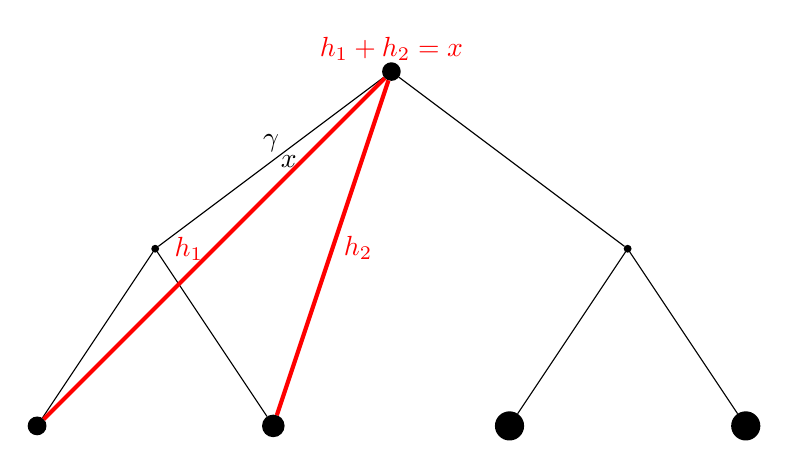
\begin{tikzpicture}
        [scale=1.5,
        level/.style={sibling distance=4cm/#1},
        vertex/.style={circle,fill=black,minimum size=1mm,inner sep=0pt,outer sep=0pt}]
        
        % Nodes
        \node[vertex] (x) {$v$}
            child {node[vertex] (c1) {} 
                child{ node[vertex] (a) {$a$} } 
                child{ node[vertex] (b) {$b$}}
                edge from parent node[above] {$\gamma$} node[right] {$x$}
                }
            child {node[vertex] (c2) {}
                child{ node[vertex] (c1') {$c_1$}} 
                child{ node[vertex] (c2') {$c_2$}}
                edge from parent node[above] {}
                };
        % Edges
        \draw[line width=1.5pt,red] (x) -- node[left] {$h_1$} (a);
        \draw[line width=1.5pt,red] (x) -- node[right] {$h_2$} (b);
        \draw[line width=1.5pt,red] (x) -- node[above] {$h_1 + h_2 = x$} (x);
        
        \end{tikzpicture}
    \caption{Figure for the proof of \cref{prop:3-cyc11}, case \eqref{case:2}. A $3_2$-cycle quartet network with internal cut edge contracted to length 0, other edge probabilities $h_1, h_2, x$, and hybridization parameter $\gamma$.}
    \label{fig:proof_case_2}
\end{figure}

\end{document}